\documentclass[simplex.tex]{subfiles}
% NO NEED TO INPUT PREAMBLES HERE
% packages are inherited; you can compile this on its own

\onlyinsubfile{
\title{NeuroData SIMPLEX Report: Subfile}
}

\begin{document}
\onlyinsubfile{
\maketitle
\thispagestyle{empty}

The following report documents the progress made by the labs of Randal~Burns and Joshua~T.~Vogelstein at Johns Hopkins University towards goals set by the DARPA SIMPLEX grant.

%%%% Table of Contents
\tableofcontents

%%%% Publications
\bibliographystyle{IEEEtran}
\begin{spacing}{0.5}
\section*{Publications, Presentations, and Talks}
%\vspace{-20pt}
\nocite{*}
{\footnotesize	\bibliography{simplex}}
\end{spacing}
%%%% End Publications
}

\subsection{Randomer Forest (RerF)}
Random Forest (RF) remains one of the most widely used general purpose
classification methods, due to its tendency to perform well in a variety of
settings. One of its main limitations, however, is that it is restricted to
only axis-aligned recursive partitions of the feature space. Consequently, RF
is particularly sensitive to the orientation of the data. Several studies have
proposed “oblique” decision forest methods to address this limitation. However,
the ways in which these methods address this issue compromise many of the nice
properties that RF possesses. In particular, unlike RF, these methods either
don’t deal with incommensurate predictors, aren’t well-adapted to problems in
which the number of irrelevant features are overwhelming, have a time and space
complexity significantly greater than RF, or require additional hyperparameters
to be tuned, rendering training of the classifier more difficult. Additionally,
oblique methods tend to be more sensitive to data corruption than RF is. Our
proposed method, which we call RerF, seeks to address these limitations. 	

Most recently, we performed simulations in which we artificially rotated,
scaled, 
rotated~+~scaled (labeled ``affine'' in figure~\ref{fig:RefF1}), and corrupted two
simulated datasets. The results demonstrate that both RerF and another existing
oblique method called RR-RF are more sensitive to scaling and corruption of the
data than is RF. The variants of these two methods that use rank
transformations to rescale the data first, called RerF(r) and RR-RF(r), become
significantly more robust to scale and corruption. While rank transformation is
not the only scale normalizing method (z-scoring and forcing all values to be
between $[0,1]$ are others), it is the only one that simultaneously helps against
data corruption. Across all simulation settings, RerF(r) is the overall best.

\begin{figure}[h!]
\begin{cframed}
\centering
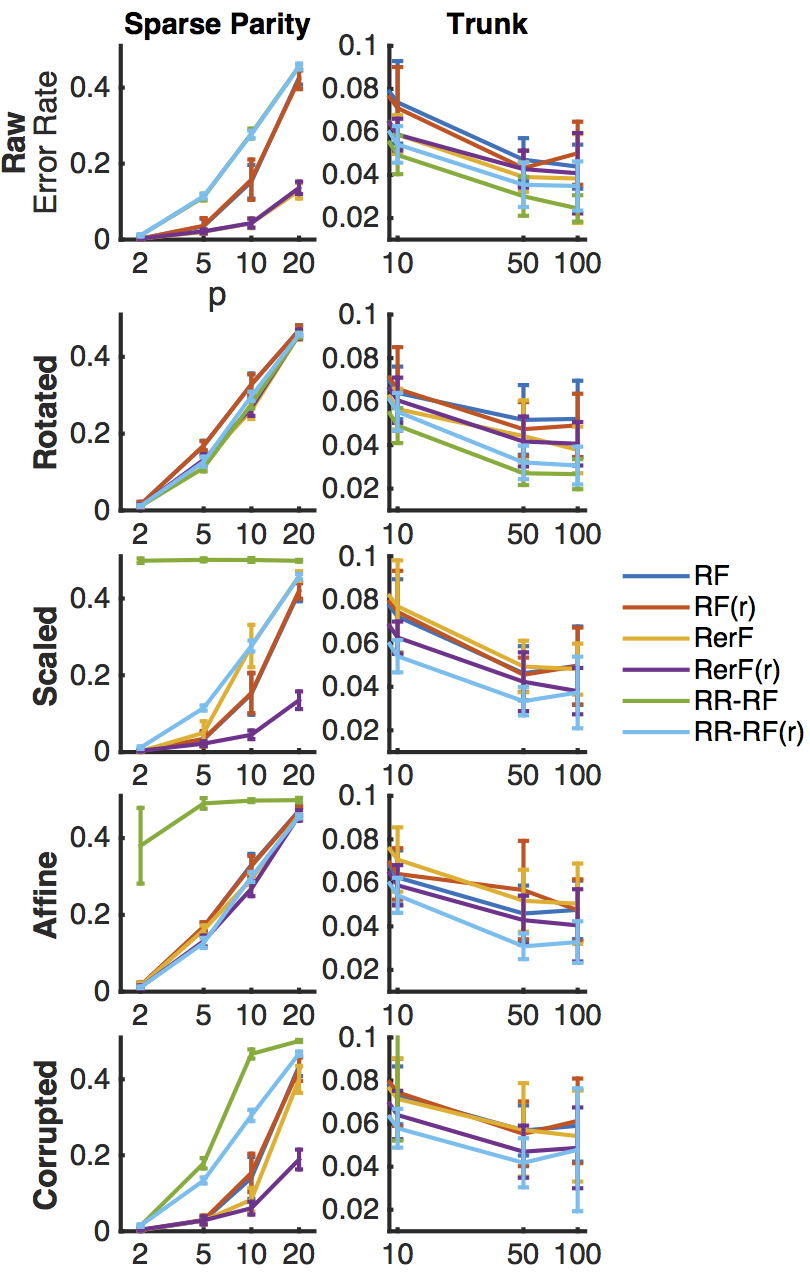
\includegraphics[height=0.5\textheight]{./figs/RefF1.png}
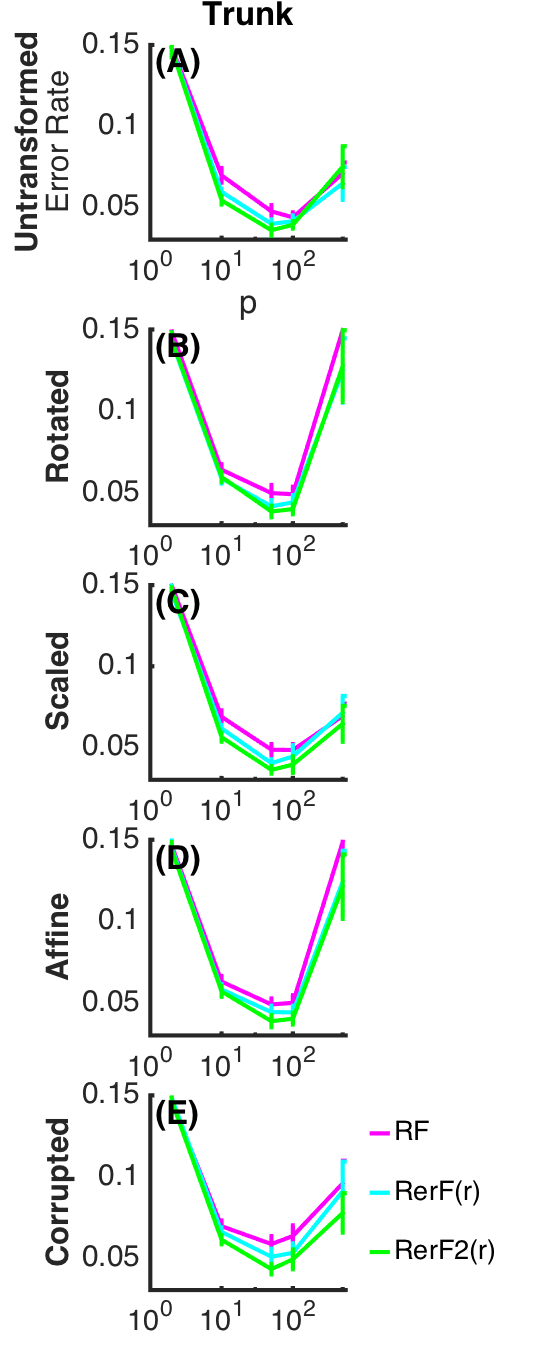
\includegraphics[height=0.5\textheight]{./figs/RefF2.png}
\caption{
 Randomer Forest Comparisons
}
\label{fig:RefF1}
\end{cframed}
\end{figure}

We are developing an R implementation of the RerF algorithm in order to make it
faster and more easily distributable.  The Rerf algorithm requires a random
rotation of data at each node during the tree creating process, but this
rotation of data at each node increases memory requirements and both training
and testing times.  So, the initial R implementation will instead rotate the
sample data once prior to creating a tree instead of at each node in the tree.
This will still increase the same factors but not to the same degree.  Initial
tests show that this single rotation per tree yields benefits similar to the
per node rotation.

The classification performance of RerF2 using the R implementation is similar
to the performance of the original RerF2 implemented in MATLAB, but the
observed differences are greater than can be explained by the use of different
randomization algorithms.  Both implementations are being analyzed to determine
the source of this observed variability.

\begin{figure}[h!]
\begin{cframed}
\centering
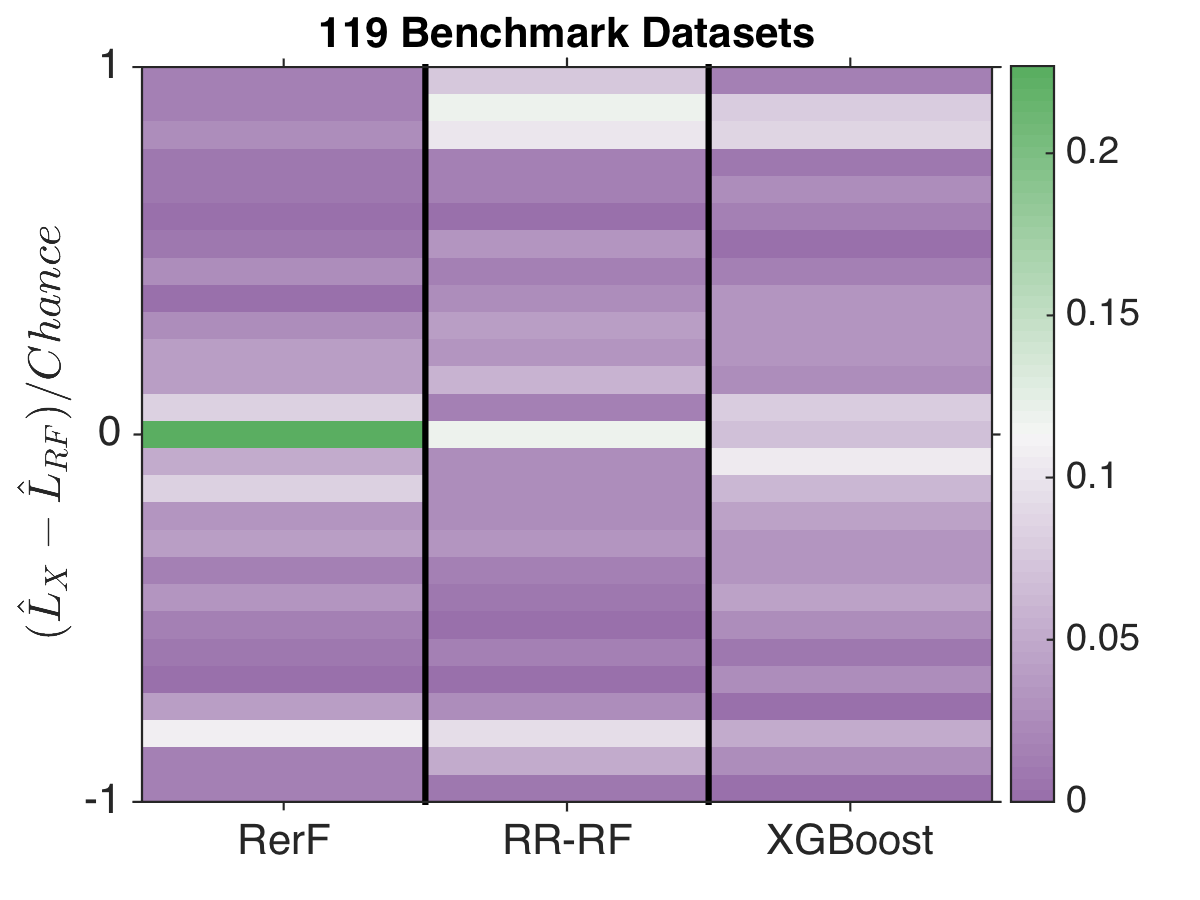
\includegraphics[height=0.5\textheight]{./figs/rerF_benchmark.png}
\caption{
Classification performances of RF, RerF, RR-RF, and XGBoost were
compared on 119 benchmark datasets. RR-RF is identical to RF except that
the data is randomly rotated prior to building each tree. XGBoost is a
computationally efficient implementation of gradient boosted trees and
has been the winner of many recent Kaggle competitions. For each
dataset, for each algorithm, error was subtracted by that of RF and
normalized by the chance probability of error. Therefore, a negative
value indicates that an algorithm had a lower error rate than RF. These
normalized relative errors were then binned and the counts in each bin
were computed. The y-axis represents the bins. Color indicates how many
times the normalized relative error of an algorithm fell into a
particular bin. For instance, the figure shows that RerF had a
normalized relative error 0.05 to 0.10 less than that of RF on
approximately 15 datasets. The ``0 to 0'' bin indicates the number of
times the normalized relative error was exactly 0. Overall the figure
indicates that RerF rarely loses to RF by much and frequently does
substantially better. RR-RF and XGBoost, on the other hand, frequently
perform worse than RF by a large margin.
}
\label{fig:RefF3}
\end{cframed}
\end{figure}

%\begin{figure}[h!]
%\begin{cframed}
%\centering
%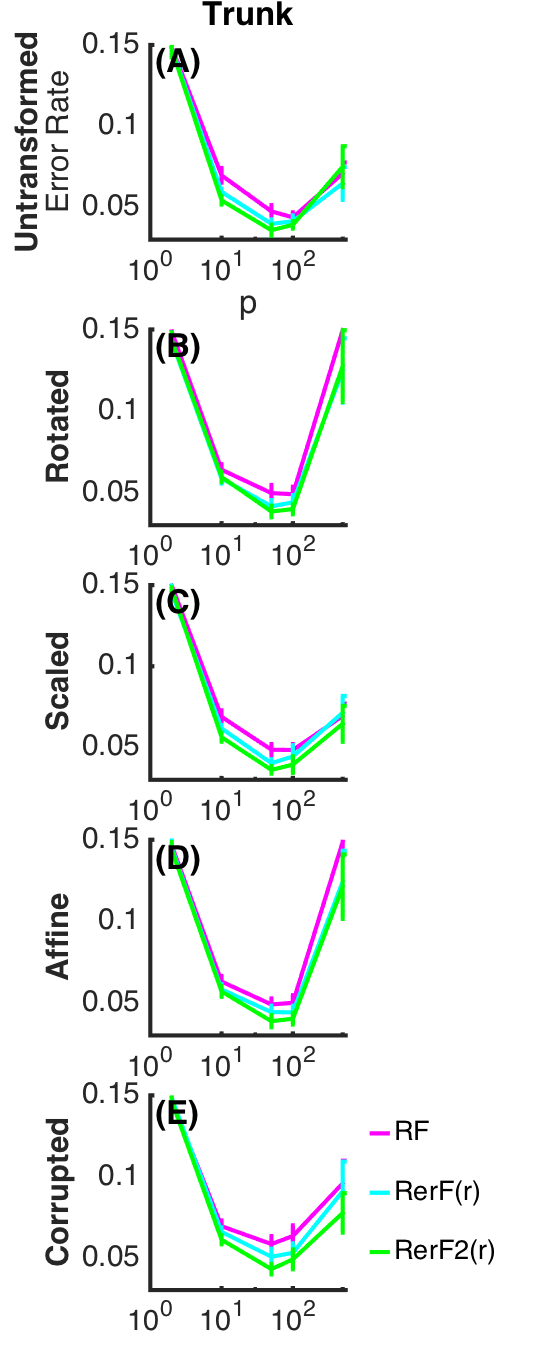
\includegraphics[height=0.5\textheight]{./figs/RefF2.png}
%\caption{
% Randomer Forest Comparisons
%}
%\label{fig:RefF2}
%\end{cframed}
%\end{figure}




\end{document}
